% !TEX root = ../main.tex
\section{Discussion} \label{sec:discussion}

\subsection{Intended Uses}
Uses for this dataset are varied and rich. Researchers could undertake a number
of machine-learning and predictive analyses to predict the likelihood of
officer misconduct from data. For example, this data and other linked data
could be used to assess an officer's likelihood of misconduct on the basis of
her demographic traits and experience, her assigned unit history, her award and
promotion history and more. As noted earlier, scholars have already used a
version of our underlying data for simple regressions designed to investigate
the correlation between complaints against officers, their likelihood of being
sued, and their likelihood of leaving the force \cite{Rozema19}. 

With the ability to link many varied sources of data, researchers could use
supervised learning analysis to refine the ability to predict officer
misconduct. Scholars have already begun to use machine learning to predict
police shootings using confidential internal data from an individual police
department \cite{Helsby18}.

This dataset can also be used by researchers who study social networks and
policing. Complaint data can be used to reconstruct the police officer social
and professional networks, by drawing connections between officers who are
listed together on a complaint. These networks are of interest in and of
themselves, but can also be used to investigate the dynamic patterns of officer
wrongdoing along such police networks \cite{Roithmayr16}. Existing research has used the complaint
data to identify such patterns and to investigate whether pairs of officers
connected on a network are more likely to have been accused of misconduct \cite{Ouellet19}.

Among several tasks, we can use the CPD dataset to perform network analysis.
\textcolor{red}{Should cite policing papers who do network analysis?}. For
example, we can use the \texttt{complaints\_officers.csv} data to construct an
undirected graph $\mathcal{G} = \{\mathcal{V}, \mathcal{E}\}$, in which
$\mathcal{V}$ is the set of nodes --- officers appearing in at least one
complaint, and $\mathcal{E}$ the set of edges --- where an edge is present
whenever two officers appeared on the same complaint. Moreover, we can link the
complaints to the \texttt{tactical\_response\_reports.csv} file, to consider
also the subgraph of officers who were also listed in a TRR. We report summary
for the corresponding graphs in \Cref{tab:stats_graphs}. Here, we consider any
complaint available to form an edge, but we only consider TRRs filed after
January 1st 2004, and before December 1st 2015.

\begin{table}[h]
\begin{tabular}{c|c|c|c|c|c|c|c|}
\cline{2-8}
                                                & $|\mathcal{G}|$ & $|\mathcal{E}|$ & \textit{Avg. degree} & \textit{Triangles} & \textit{Max clique} & \textit{LCC} & \textit{\# Is. nodes} \\ \hline
\multicolumn{1}{|c|}{\textit{\textbf{All}}}     & $14{,}372$      & $106{,}701$     & $14.85$              & $361{,}878$        & $64$                & $13{,}950$   & $0$                   \\ \hline
\multicolumn{1}{|c|}{\textit{\textbf{In TRRs}}} & $4{,}105$       & $22{,}064$      & $10.75$              & $44{,}786$         & $28$                & $3{,}822$    & $225$                 \\ \hline
\end{tabular} \label{tab:stats_graphs}
\caption{Summary statistics for the complaints network graph, and the subgraph
of officers in TRRs. Here LCC is the largest connected components, and Is.
nodes is the number of isolated nodes.}\label{tab:network}
\end{table}

\begin{figure}[t!] 
	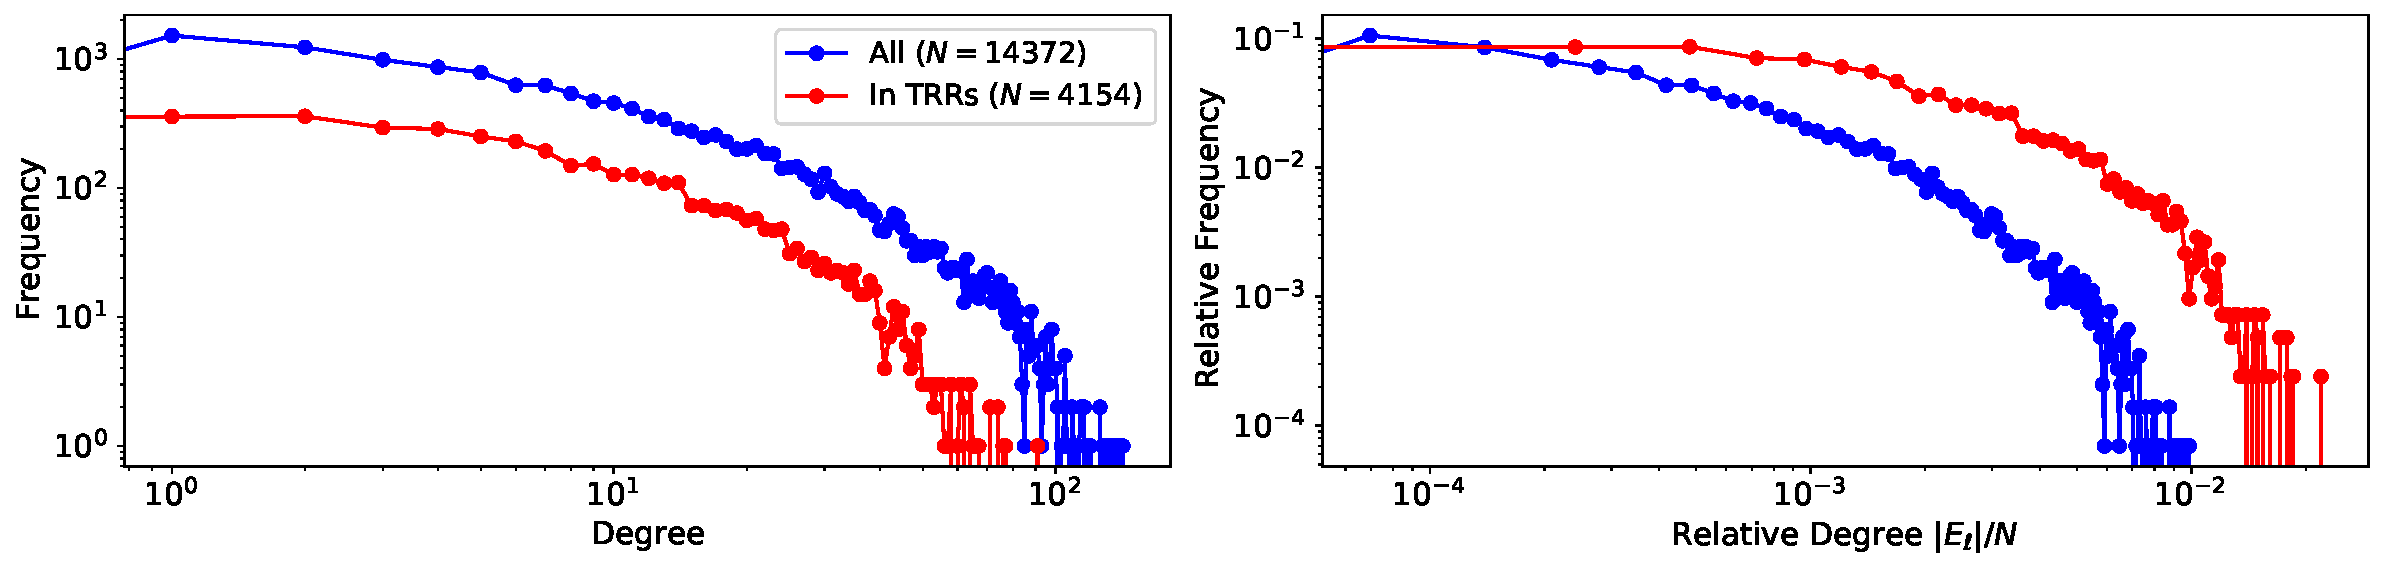
\includegraphics[width=\textwidth]{figs/degree_distribution} 
	\caption{Degree distribution for the complaints network.}
\label{fig:degree_distribution}
\end{figure}

\begin{figure}[t!] 
	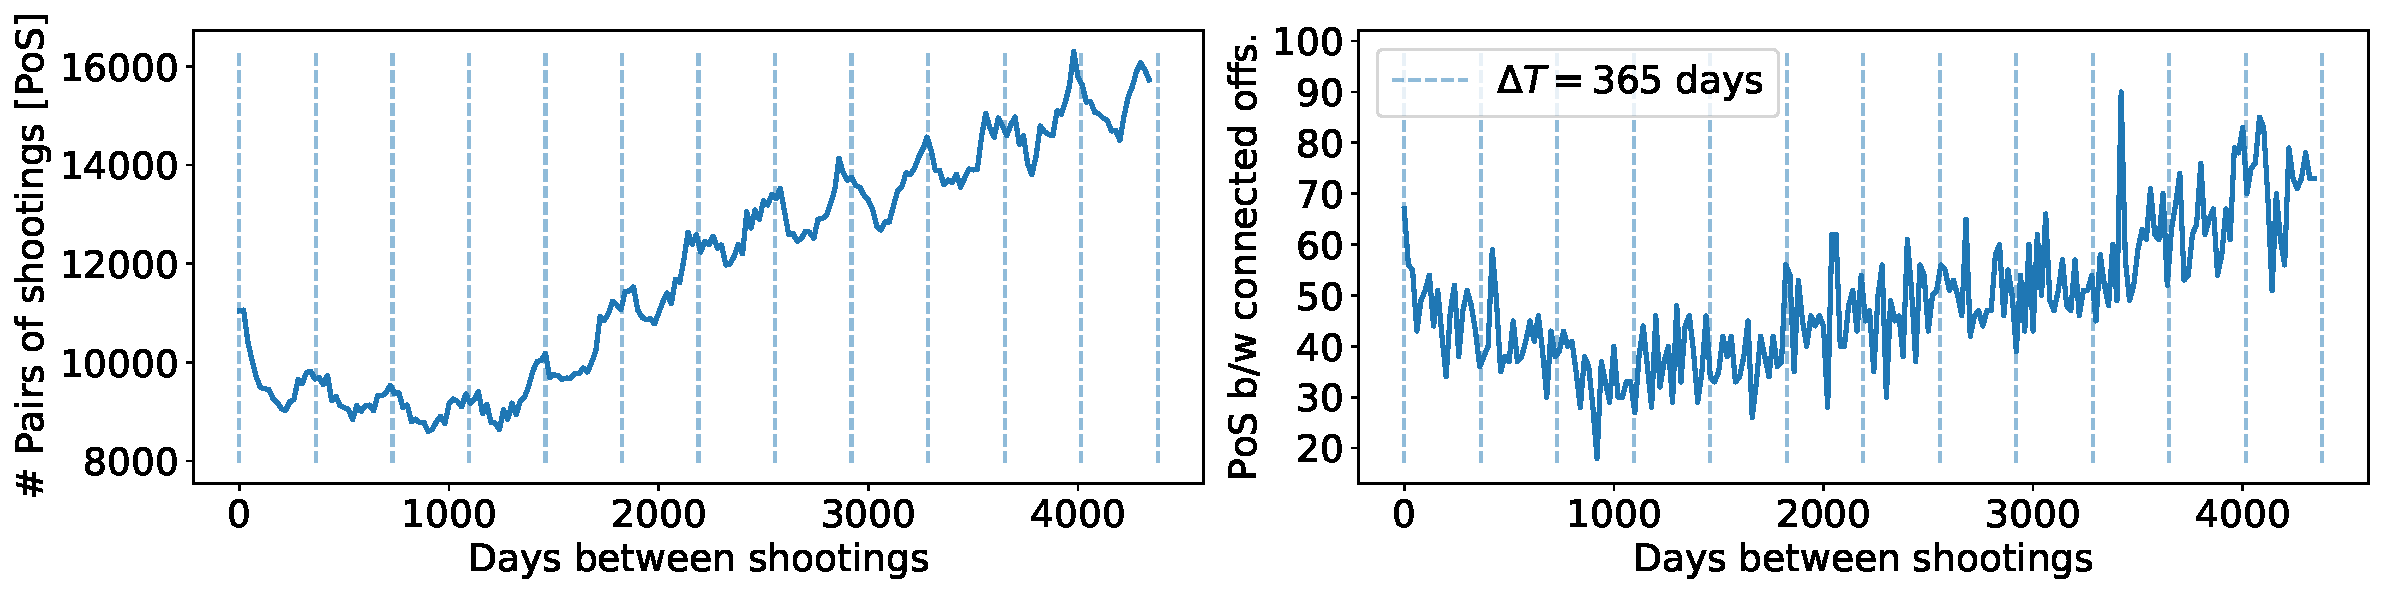
\includegraphics[width=\textwidth]{figs/intrashooting_times} 
	\caption{Intrashooting times between pairs of shootings.}
\label{fig:intrashooting_time}
\end{figure}

Finally, this dataset could be used to track the effects of new disciplinary
practices, new training techniques, and new oversight on complaints and use of
force. A working paper explores, for example, whether civilians filed fewer
complaints about officers' force in the wake of the Department of Justice
investigation of the Chicago Police Department \cite{Travers20}. 

\subsection{Ethical Considerations}
Recent work on algorithmic fairness focuses on the potential for racially
biased data to produce racially biased results
\cite{veale2018fairness,sloane2019ai,d2020fairness}.  This research suggests
that race shapes data collection in criminal justice, in at least two ways that
are likely to affect data collection on black officers. First, beginning back
in the 1960s, black officers are more likely to be assigned to black
neighborhoods and/or to neighborhoods where police interaction is more
pervasive \cite{Kuykendall80}. Given an increased frequency of interaction,
officers assigned to these neighborhoods may be statistically more likely to be
the subject of complaints \cite{Kane06}. 

Second, owing to cognitive bias, complainants may be more likely to file a
complaint against black officers, either alone or in pairs. This racial
asymmetry in the collection of complaint data may well produce, for example,
racially biased predictions of police misconduct. Relatedly, because our
dataset may be used to explore predictive policing of the police, black
officers may be unfairly and disproportionately identified to be at higher risk
of misconduct \cite{veale2018fairness,sloane2019ai,d2020fairness,Wood19}. 

\subsection{Limitations and Future Work}
Using civilian and administrator complaint data to study actual police
misconduct (and not perceived misconduct) inevitably faces significant
questions about validity. At least one study has found that because of flaws in
police record keeping and categorization, the practice of using complaints to
measure police behavior suffers from ``serious measurement flaws, and does not
provide a valid and reliable basis for research purposes...'' \cite{Hickman16} Even so, other
research finds a strong correlation between civilian-filed complaints against
officers and internal complaints against the same officers filed by other
officers or supervisors \cite{Lersch00}. Whatever the truth of the matter, the dataset could be
strengthened by adding more objective measures of misconduct, for example, data
on individual officer misconduct from oversight agencies.

Use of this dataset for network research faces a particular set of limitations.
To wit, researchers who use complaint data to generate social networks must
acknowledge that the co-listing of two officers on a complaint is a very coarse
and incomplete proxy for a professional network relationship and for the
exposure to another officer’s misconduct. Data on partner assignment and
dispatch data would more accurately reflect officer relationships and their
exposure to misconduct. 

In general, future work should focus on integrating into this dataset as many
objective sources of data on individual officers as possible. Objective data
could include information about adverse incident histories, officer discipline
histories, counseling interventions, domestic violence incidents, weapons
violations, sustained complaints, lawsuit settlements. Additional information
about officer activities could include partner assignments, dispatch
information, arrest and stop information. 

In addition, information about the units to which officers are assigned,
including the unit's disciplinary history, leadership turnover, partner
assignment policies, could be easily integrated to shed even more light on
policing and police misconduct. At the department level, the 2016 Department of
Justice report of its investigation of the Chicago Police Department can supply
additional information on not just the department but its subunits and
individual officers.
